% \iffalse
%<*internal>
\begingroup
\input docstrip.tex
\keepsilent
\usedir{tex/latex/pdffill}
\let\MetaPrefix\relax
\preamble
_____________________________________________________________
The pdffill package for LaTeX
Copyright (c) 2011 Kazuki Maeda <kmaeda@kmaeda.net>

Distributable under the MIT License:
http://www.opensource.org/licenses/mit-license.php

\endpreamble
\askforoverwritefalse

\let\MetaPrefix\DoubleperCent
\generate{\file{pdffill.sty}{\from{pdffill.dtx}{package}}}
\endgroup
%</internal>
%
\NeedsTeXFormat{LaTeX2e}
%<package>\ProvidesPackage{pdffill}
%<driver>\ProvidesFile{pdffill.dtx}
%<driver|package>  [2011/05/08 fill in PDF]
%<*driver>
\documentclass{ltjsarticle}
\usepackage{doc}
\usepackage{metalogo}
\usepackage[unicode,hypertexnames=false,bookmarks=false,colorlinks,citecolor=blue,linkcolor=blue,urlcolor=blue]{hyperref}
\usepackage{pdffill}
\usepackage{unicode-math}
\setmainfont{TeX Gyre Termes}
\setsansfont{TeX Gyre Heros}
\setmonofont{Inconsolata-zi4}
\setmathfont{XITSMath}
\addtolength{\textwidth}{-1in}
\addtolength{\oddsidemargin}{1in}
\addtolength{\evensidemargin}{1in}
\addtolength{\marginparwidth}{1in}
\setlength\marginparpush{0pt}
\CodelineNumbered
\begin{document}
  \DocInput{\jobname.dtx}
\end{document}
%</driver>
%
% \fi
%
% \MakeShortVerb{\|}
% ^^A l3doc style
% \makeatletter
% \def\macro{\begingroup
%    \catcode`\\12
%    \catcode`\_12
%    \MakePrivateLetters \m@cro@ \iftrue}
% \makeatother
% \def\theCodelineNo{\textcolor[gray]{0.5}{\sffamily\tiny\arabic{CodelineNo}}}
%
% \title{\texttt{pdffill} パッケージ}
% \author{前田一貴}
% \maketitle
% \tableofcontents
%
% \section{概要}
%
% 申請書や報告書といった事務書類を作成するとき,慣れない Word や Excel の様式を送ら
% れて編集する必要に迫られることが多いです.特にある程度の長さの文章を記述する欄があ
% る場合,Word や Excel では無様な仕上がりになってしまったり,枠が崩れてしまったり,
% ページ数が不意に増えたりしてイライラします(使い方が下手なせいかもしれないが).
% あげくの果てに記入して保存したファイルを修正のためにもう一度開こうとしたらクラッシュ
% した日には……(←実体験).
%
% |pdffill| は使い慣れた \LaTeX で美しく事務書類を作成するためのパッケージです.
% 目標は科研費 \LaTeX\footnote{\url{http://osksn2.hep.sci.osaka-u.ac.jp/~taku/kakenhiLaTeX/}}
% の方法を一般化することです.
%
% \section{依存パッケージ}
%
% |tikz|, |expl3|, |xparse|, |pdfpages|.
% さらに,日本語を書くために,\LuaTeX ならば \LuaTeX-ja
% \footnote{\url{http://sourceforge.jp/projects/luatex-ja/wiki/FrontPage}},
% \XeTeX ならば ZXjatype
% \footnote{\url{http://zrbabbler.sp.land.to/zxjatype.html}}
% を用意して下さい.
% なお,このドキュメントでは \LuaTeX-ja を用いています.
%
% \section{とりあえず使ってみよう}
%
% 細かいことを書く前にまずは使い方を見てみましょう.
% 例として,次ページにあるような申請書に記入することを考えます.
%
% 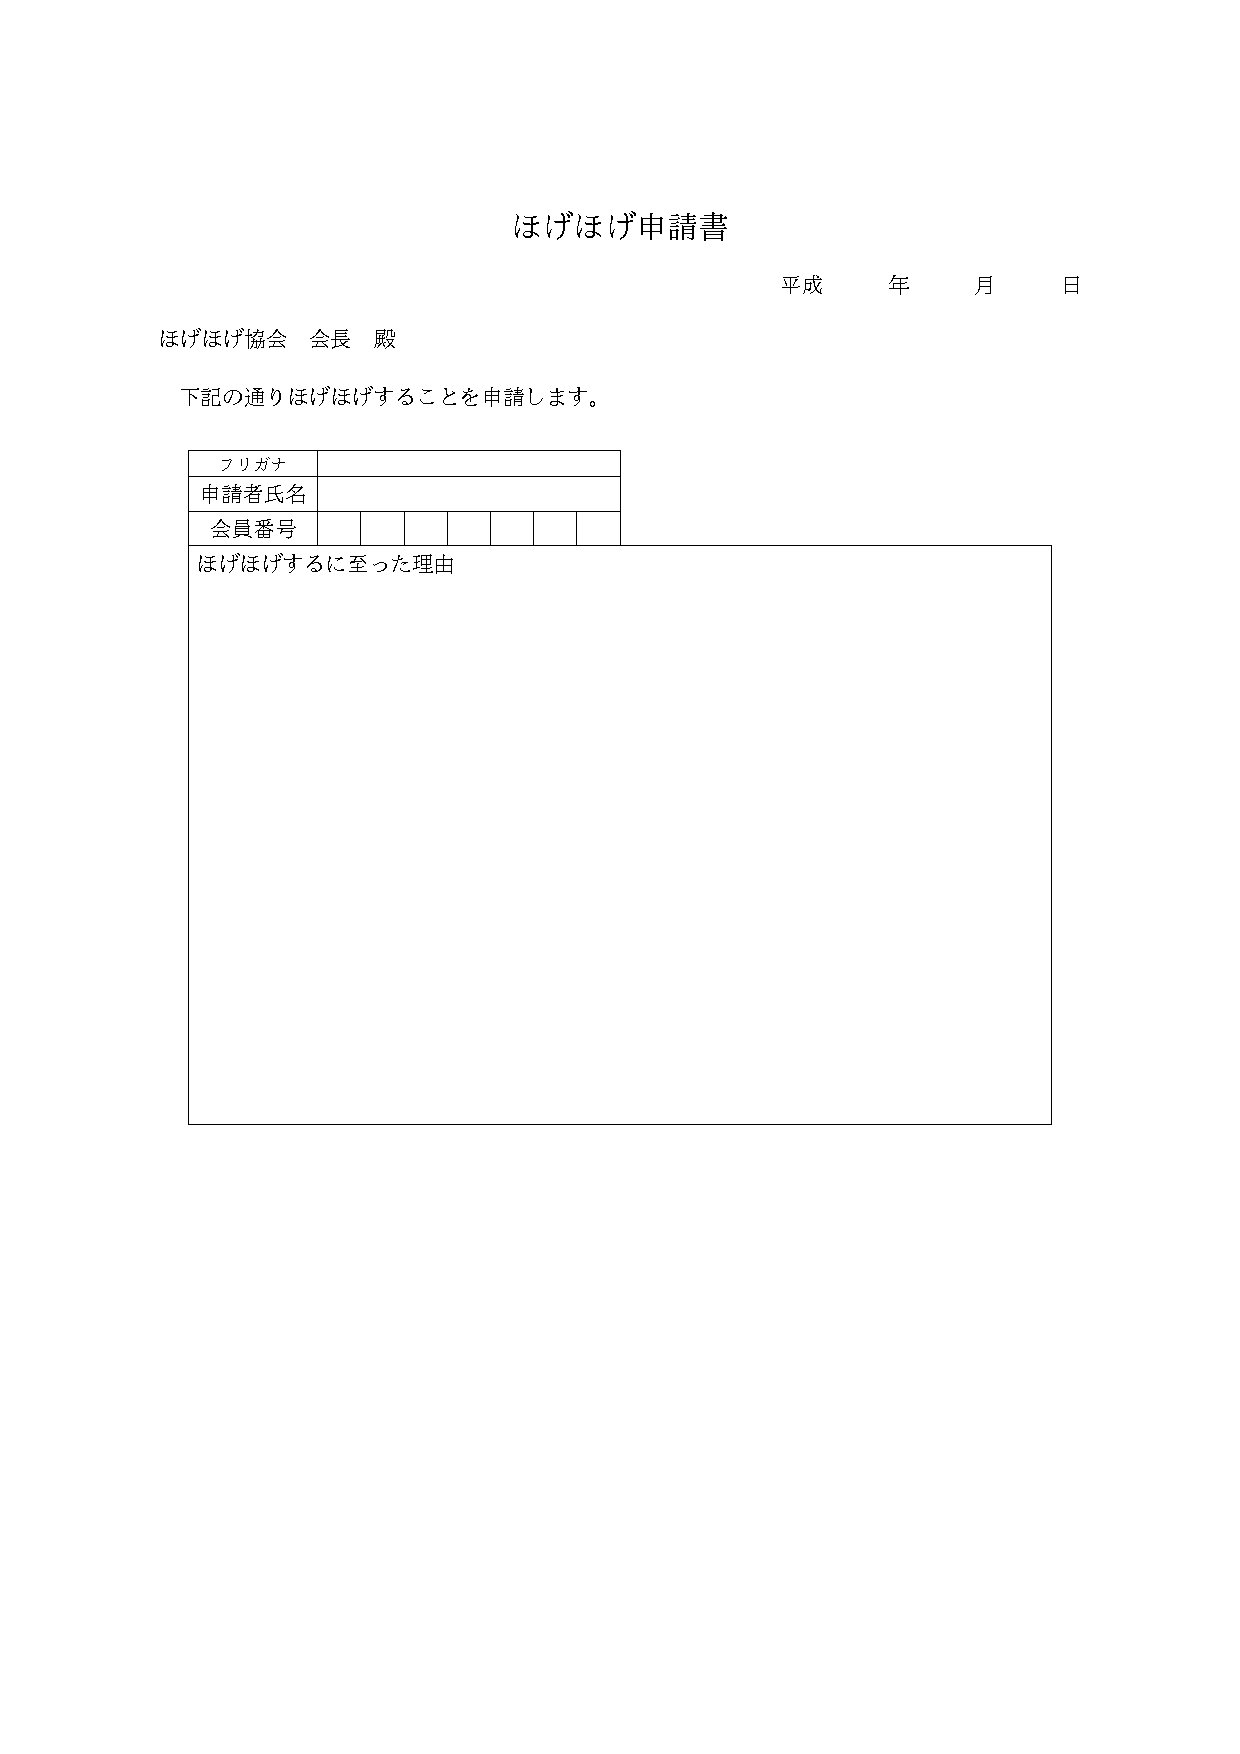
\includepdf{sampleform}
%
% この申請書のファイル名を |sampleform.pdf| とします.
% ここでは \LuaTeX-ja を用いることとし,次のように書いたファイルを
% 同じディレクトリに用意しましょう.
% \begin{quote}
% \begin{verbatim}
% \documentclass{ltjsarticle}
% \usepackage{pdffill}
% %% ここに日本語関連のパッケージの読み込み・設定を書く
% \begin{document}
% \pfdefaultoption{grid,draft}
% \pdffill{sampleform}{}
% \end{document}
% \end{verbatim}
% \end{quote}
%
% これを |lualatex| コマンドでコンパイルすると次ページのような出力が得られます
% (2011/10/14 以降の \LuaTeX-ja をインストールしておく必要あり).
%
% \noindent {\bfseries (注意)}PDF ビューワによってはこれで描かれるグリッドが
% 意図通り点線にならずに,見辛くなってしまうことがあるようです.
%
% 出力を見ながら |\pdffill{sampleform}{}| の部分を次のように変えてみましょう.
% \long\def\picturecommand{
%   \pfnode[right] (13.75, 24.85) {\splitboxes{14.5mm}{{23}{5}{9}}}
%   \pfnode[right] (5.6, 21.85) {\footnotesize ホゲ タロウ}
%   \pfnode[right] (5.6, 21.3) {保毛 太郎}
%   \pfnode[right] (5.38, 20.7) {\splitboxes{7.3mm}{1234567}}
%   \pfnode[below right,text width=44\zw] (3.3, 20) {\parindent=1\zw\par
%     これまでに多くの場でほげほげの経験を積み,その結果あらゆる場面でほげほげする能力を
%     身に付けることができました.
%     この能力をより広く社会で生かしていくためには,貴協会でほげほげすることが
%     何よりも効果的であると判断しました.
%     申請が認められた後には,全世界でほげほげするほげほげツアーを実施し,
%     さらにほげほげをほげほげしていく所存でほげほげ.
%
%     ほげほげほげほげほげほげほげほげほげほげほげほげほげほげほげほげほげほげほげ
%     ほげほげほげほげほげほげほげほげほげほげほげほげほげほげほげほげほげほげほげ
%     ほげほげほげほげほげほげほげほげほげほげほげほげほげほげほげほげほげほげほげ
%     ほげほげほげほげほげほげほげほげほげほげほげほげほげほげほげほげほげほげほげ
%     ほげほげほげほげほげほげほげほげほげほげほげほげほげほげほげほげほげほげほげ
%     ほげほげほげほげほげほげほげほげほげほげほげほげほげほげほげほげほげほげほげ
%     ほげほげほげほげほげほげほげほげほげほげほげほげほげほげほげほげほげほげほげ
%     ほげほげほげほげほげほげほげほげほげほげほげほげほげほげほげほげほげほげほげ
%     ほげほげほげほげほげほげほげほげほげほげほげほげほげほげほげほげほげほげほげ
%     ほげほげほげほげほげほげほげほげほげほげほげほげほげほげほげほげほげほげほげ
%     ほげほげほげほげほげほげほげほげほげほげほげほげほげほげほげほげほげほげほげ
%     ほげほげほげほげほげほげほげほげほげほげほげほげほげほげほげほげほげほげほげ
%     ほげほげほげほげほげほげほげほげほげほげほげほげほげほげほげほげほげほげほげ
%     ほげほげほげほげほげほげほげほげほげほげほげほげほげほげほげほげ!
%   }
% }
%
% \begin{quote}
% \begin{verbatim}
% \pdffill{sampleform}{
%   % 日付
%   \pfnode[right] (13.75, 24.85) {\splitboxes{14.5mm}{{23}{5}{9}}}
%   % 名前のフリガナ
%   \pfnode[right] (5.6, 21.85) {\footnotesize ホゲ タロウ}
%   % 名前
%   \pfnode[right] (5.6, 21.3) {保毛 太郎}
%   % 会員番号
%   \pfnode[right] (5.38, 20.7) {\splitboxes{7.3mm}{1234567}}
%   % 申請理由
%   \pfnode[below right,text width=44\zw] (3.3, 20) {\parindent=1\zw\par
%     これまでに多くの場でほげほげの経験を積み,その結果あらゆる場面でほげほげする
%     能力を身に付けることができました.
%     この能力をより広く社会で生かしていくためには,貴協会でほげほげすることが
%     何よりも効果的であると判断しました.
%     申請が認められた後には,全世界でほげほげするほげほげツアーを実施し,
%     さらにほげほげをほげほげしていく所存でほげほげ.
%
%     ほげほげほげほげほげほげほげほげほげほげほげほげほげほげほげほげほげほげほげ
%     (以下略)
%   }
% }
% \end{verbatim}
% \end{quote}
%
% これで次々ページの出力が得られます.さらに \verb|\pfdefaultoption{grid,draft}| を
% コメントアウトすれば完成です.
%
% \pdffill[grid,draft]{sampleform}{}
%
% \pdffill[grid,draft]{sampleform}{\picturecommand}
%
% \pdffill{sampleform}{\picturecommand}
%
%
% \section{ユーザ用コマンドの説明}
%
% そのうち書きます…….
%
% \section{実装}
%
% \subsection{パッケージの読み込み}
%
% まず,必要なパッケージを読み込み,明るい未来のために |\ExplSyntaxOn| します.
%    \begin{macrocode}
\RequirePackage{tikz}
\RequirePackage{expl3,xparse}
\ExplSyntaxOn
\RequirePackage{pdfpages}
%    \end{macrocode}
%
% \subsection{オプションの定義と変数の用意}
%
% \begin{macro}{\l_pf_page_int}
% \begin{macro}{\l_pf_draft_bool}
% \begin{macro}{\l_pf_draftcolor_tl}
% \begin{macro}{\l_pf_grid_bool}
% \begin{macro}{\l_pf_gridcolor_tl}
% \begin{macro}{\l_pf_tics_dim}
% \begin{macro}{\l_pf_gridstep_int}
% \begin{macro}{\l_pf_labelstep_int}
% |\pdffill| コマンドのオプションを |l3keys| を用いて定義します.
%    \begin{macrocode}
\keys_define:nn {pdffill} {
  page       .int_set:N  = \l_pf_page_int,
  draft      .bool_set:N = \l_pf_draft_bool,
  draft      .default:n  = true,
  draftcolor .tl_set:N   = \l_pf_draftcolor_tl,
  grid       .bool_set:N = \l_pf_grid_bool,
  grid       .default:n  = true,
  gridcolor  .tl_set:N   = \l_pf_gridcolor_tl,
  tics       .dim_set:N  = \l_pf_tics_dim,
  gridstep   .int_set:N  = \l_pf_gridstep_int,
  labelstep  .int_set:N  = \l_pf_labelstep_int,
}
%    \end{macrocode}
% \end{macro}
% \end{macro}
% \end{macro}
% \end{macro}
% \end{macro}
% \end{macro}
% \end{macro}
% \end{macro}
% \begin{macro}{\g_pf_defaultoption_tl}
% \begin{macro}{\l_pf_tmpx_dim}
% \begin{macro}{\l_pf_tmpy_dim}
% \begin{macro}{\l_pf_gridstep_dim}
% その他,必要な変数を定義します.
%    \begin{macrocode}
\tl_new:N  \g_pf_defaultoption_tl
\dim_new:N \l_pf_tmpx_dim
\dim_new:N \l_pf_tmpy_dim
\dim_new:N \l_pf_gridstep_dim
%    \end{macrocode}
% \end{macro}
% \end{macro}
% \end{macro}
% \end{macro}
%
% \subsection{デフォルト値}
%
% 上で準備した変数のデフォルト値を設定します.
%    \begin{macrocode}
\int_set:Nn \l_pf_page_int      \c_one
\tl_set:Nn  \l_pf_draftcolor_tl {red}
\tl_set:Nn  \l_pf_gridcolor_tl  {blue!40}
\dim_set:Nn \l_pf_tics_dim      {2mm}
\int_set:Nn \l_pf_gridstep_int  \c_one
\int_set:Nn \l_pf_labelstep_int \c_ten
%    \end{macrocode}
%
% \subsection{ユーザ用コマンドの定義}
%
%
% \begin{macro}{\pfdefaultoption}
% |\pdffill| のオプションのデフォルト値を設定するコマンドです.
% |\g_pf_defaultoption_tl| に指定された値をセットするだけです.
%    \begin{macrocode}
\ProvideDocumentCommand \pfdefaultoption { m } {
  \tl_gset:Nn \g_pf_defaultoption_tl {#1}
}
%    \end{macrocode}
% \end{macro}
% \begin{macro}{\pfnode}
% |\pdffill| 中で使用するための Ti{\itshape k}Z の |\node| に相当するコマンドです.
% このコマンドを用いることで,|draft| オプションが機能します.
%    \begin{macrocode}
\ProvideDocumentCommand \pfnode { O{} u(u,u) +m } {
  \bool_if:NTF \l_pf_draft_bool {
    \node[#1,draw=\l_pf_draftcolor_tl] at (#3, #4) {#5};
    \draw[draw=\l_pf_draftcolor_tl,fill=\l_pf_draftcolor_tl]
    (#3, #4) circle (0.5mm);
  } {
    \node[#1] at (#3, #4) {#5};
  }
}
%    \end{macrocode}
% \end{macro}
% \begin{macro}{\pdffill}
% このパッケージにおいて最も重要なコマンドです.
% まずはオプションの処理をします.
%    \begin{macrocode}
\cs_generate_variant:Nn \keys_set:nn {nx}
\ProvideDocumentCommand \pdffill { O{} m +m } {
  \group_begin:
  \keys_set:nx {pdffill} {\g_pf_defaultoption_tl,#1}
%    \end{macrocode}
% \begin{macro}{\l_pf_picturecommand_tl}
% |\includepdf| に渡す |picturecommand| を定義します.
% 実際には |picture| 環境ではなく |tikzpicture| 環境を使いたいので,
% |\put(0, 0)| の中にパディングなしで overlay な |tikzpicture| を入れます.
% そして,冒頭に指定されたコマンドを流し込みます.
%    \begin{macrocode}
  \tl_set:Nn \l_pf_picturecommand_tl {
    \put(0, 0){\noindent
      \begin{tikzpicture}[inner~sep=0pt,overlay]
        #3
%    \end{macrocode}
% 次に,もし |grid| オプションが指定されていたらグリッドを描きます.
%    \begin{macrocode}
        \bool_if:NT \l_pf_grid_bool {
          \dim_set:Nn \l_pf_gridstep_dim
              {1cm * \l_pf_gridstep_int}
          \draw[color=\l_pf_gridcolor_tl,densely~dotted,step=\l_pf_tics_dim]
          (0, 0) grid (\paperwidth, \paperheight);
          \draw[color=\l_pf_gridcolor_tl,densely~dotted,
            step=\l_pf_gridstep_dim,thick]
          (0, 0) grid (\paperwidth, \paperheight);
%    \end{macrocode}
% 目盛を書きます.まずは $x$ 方向.
%    \begin{macrocode}
          \dim_set:Nn \l_pf_tmpy_dim {\l_pf_gridstep_dim / 2}
          \dim_while_do:nNnn \l_pf_tmpy_dim < \paperheight {
            \dim_set:Nn \l_pf_tmpx_dim \l_pf_gridstep_dim
            \int_set_eq:NN \l_tmpa_int \l_pf_gridstep_int
            \dim_while_do:nNnn \l_pf_tmpx_dim < \paperwidth {
              \node[color=\l_pf_gridcolor_tl] at (\l_pf_tmpx_dim, \l_pf_tmpy_dim)
                   {\scriptsize \int_use:N \l_tmpa_int};
              \dim_add:Nn \l_pf_tmpx_dim \l_pf_gridstep_dim
              \int_add:Nn \l_tmpa_int \l_pf_gridstep_int
            }
            \dim_add:Nn \l_pf_tmpy_dim {\l_pf_gridstep_dim * \l_pf_labelstep_int}
          }
%    \end{macrocode}
% 同様にして $y$ 方向も書きます.
%    \begin{macrocode}
          \dim_set:Nn \l_pf_tmpx_dim {\l_pf_gridstep_dim / 2}
          \dim_while_do:nNnn \l_pf_tmpx_dim < \paperwidth {
            \dim_set:Nn \l_pf_tmpy_dim \l_pf_gridstep_dim
            \int_set_eq:NN \l_tmpa_int \l_pf_gridstep_int
            \dim_while_do:nNnn \l_pf_tmpy_dim < \paperheight {
              \node[color=\l_pf_gridcolor_tl] at (\l_pf_tmpx_dim, \l_pf_tmpy_dim)
                   {\scriptsize \int_use:N \l_tmpa_int};
              \dim_add:Nn \l_pf_tmpy_dim \l_pf_gridstep_dim
              \int_add:Nn \l_tmpa_int \l_pf_gridstep_int
            }
            \dim_add:Nn \l_pf_tmpx_dim {\l_pf_gridstep_dim * \l_pf_labelstep_int}
          }
        }
      \end{tikzpicture}
    }
  }
%    \end{macrocode}
% \end{macro}
% 最後に目的の PDF ファイルを |\includepdf| して,その上から
% |picturecommand| を描きます.
%    \begin{macrocode}
  \includepdf[pages=\int_use:N \l_pf_page_int,
              picturecommand=\l_pf_picturecommand_tl,
              fitpaper]
             {#2}
  \group_end:
}
%    \end{macrocode}
% \end{macro}
% \begin{macro}{\splitboxes}
% トークンを等間隔に配置するための簡単なコマンドです.
%    \begin{macrocode}
\cs_generate_variant:Nn \tl_if_eq_p:NN {nn}
\ProvideDocumentCommand \splitboxes { O{c} m m } {
  \tl_map_inline:nn {#3} {\hbox_to_wd:nn {#2} {
      \bool_if:nT {\tl_if_eq_p:nn {#1} {c} || \tl_if_eq_p:nn {#1} {r}} {
        \tex_hss:D
      }
      ##1
      \bool_if:nT {\tl_if_eq_p:nn {#1} {c} || \tl_if_eq_p:nn {#1} {l}} {
        \tex_hss:D
      }
    }
  }
}
%    \end{macrocode}
% \end{macro}
\endinput
